\section{Resultados Experimentales}
\label{sec:resultados}

\subsection{Experimento de proporcionalidad (Casos 3 y 4)}

Ambos casos corren con 5 tareas de $10^{7}$ unidades cada una, ventana
truncada a $10^4$ despachos (\texttt{--max-dispatches}) y quantum $Q=1000$,
sobre 30 semillas no nulas ($1, \ldots, 30$), reproducible con
\texttt{scripts/experimento\_proporcionalidad.py}. La ventana truncada es
necesaria para que la ponderación por boletos
sea observable: si se deja correr hasta que todas las tareas terminan,
\texttt{observed\_share} converge a $1/N$ para todas independientemente de
sus boletos, porque cada tarea termina consumiendo exactamente su trabajo
total sin importar cuántas veces ganó el sorteo en el camino.

El Caso 3 (Igualdad, boletos iguales) confirma que sin diferencias de
boletos el share converge a $1/5 = 0.20$ para las cinco tareas, con un error
absoluto medio de $0.000477$ sobre las 30 semillas (Tabla~\ref{tab:caso3}).

\begin{table}[htbp]
\caption{Caso 3 (Igualdad): share observado por tarea, 30 semillas}
\label{tab:caso3}
\centering
\begin{tabular}{ccccc}
\toprule
id & objetivo & media & desv. std. & error abs. \\
\midrule
1 & 0.200000 & 0.199303 & 0.003660 & 0.000697 \\
2 & 0.200000 & 0.200730 & 0.004186 & 0.000730 \\
3 & 0.200000 & 0.199740 & 0.003769 & 0.000260 \\
4 & 0.200000 & 0.200463 & 0.003250 & 0.000463 \\
5 & 0.200000 & 0.199763 & 0.003909 & 0.000237 \\
\bottomrule
\end{tabular}
\end{table}

El Caso 4 (Proporcionalidad, boletos 10/20/30/40/50) es el caso ilustrativo:
sus objetivos difieren por tarea ($1/15, \ldots, 5/15$), así que revela si el
sorteo realmente pondera por boletos y no solo distribuye de forma uniforme.
La Fig.~\ref{fig:objetivo-observado} compara el share objetivo con el
promedio observado sobre las 30 semillas, con la desviación estándar entre
semillas como barra de error; el error absoluto medio entre tareas es
$0.001104$, muy por debajo de la tolerancia del enunciado ($\leq 0.02$), y
las barras de error son minúsculas con la ventana completa de $10^4$
despachos.

\begin{figure}[htbp]
\centering
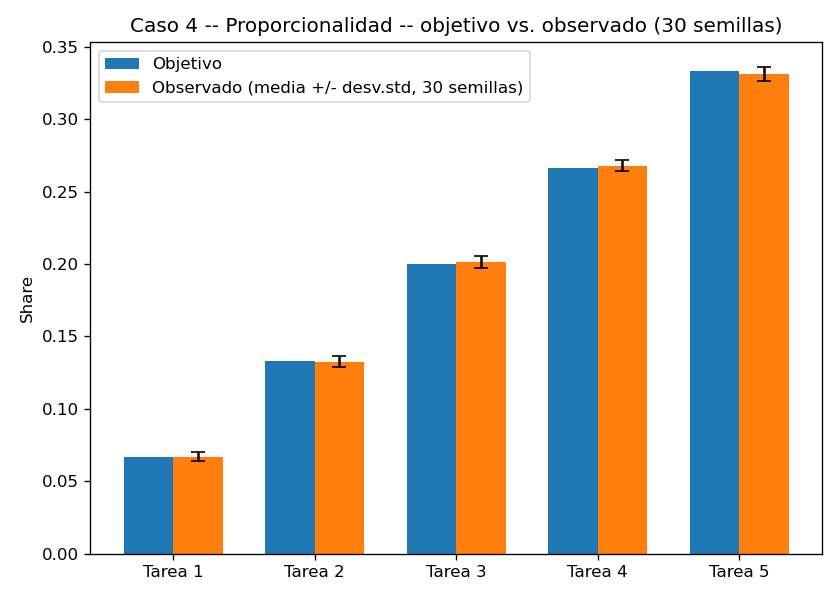
\includegraphics[width=\linewidth]{../../results/proporcionalidad/caso4_objetivo_vs_observado.png}
\caption{Caso 4 (Proporcionalidad): share objetivo vs. promedio observado
por tarea, con desviación estándar entre las 30 semillas como barra de
error. Generado por \texttt{scripts/experimento\_proporcionalidad.py}.}
\label{fig:objetivo-observado}
\end{figure}

\subsection{Análisis 1: la lotería no garantiza exactitud en ventanas cortas}

La Fig.~\ref{fig:convergencia} muestra el share acumulado de cada tarea
después de cada despacho, de una semilla representativa (\texttt{seed=1}),
desde el despacho 1 hasta el 10\,000. En los primeros cientos de despachos
las cinco líneas oscilan con amplitud grande y hasta se cruzan entre sí ---
la tarea 4 (40 boletos, objetivo $0.267$) llega a tener share $=1.0$
inmediatamente después del primer despacho, porque con una sola muestra
quien gana tiene automáticamente el 100\,\% de lo acumulado hasta ese punto.
A partir de aproximadamente el despacho 2000, cada línea se aplana en una
banda angosta alrededor de su objetivo (línea punteada) y prácticamente no
se mueve más.

\begin{figure}[htbp]
\centering
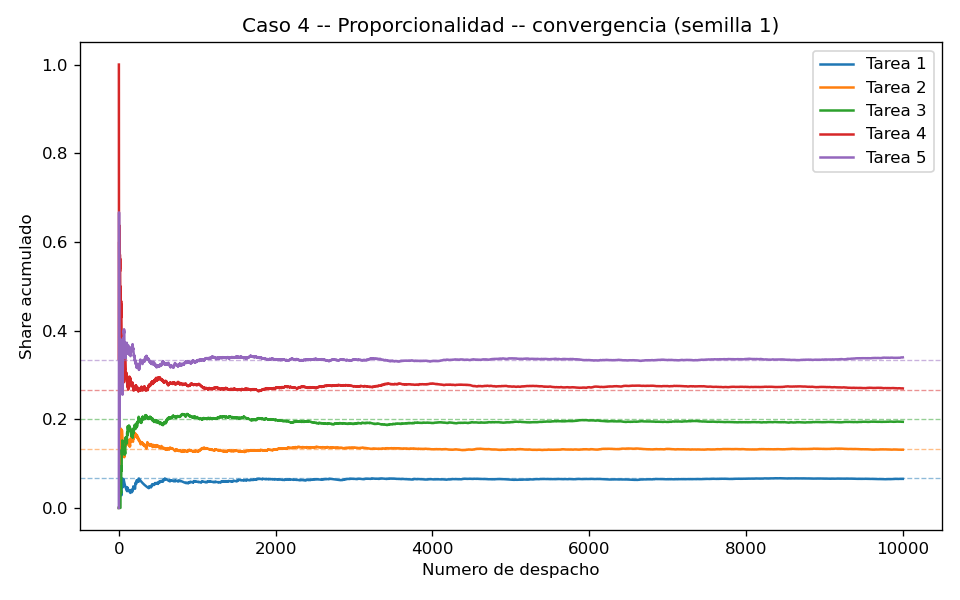
\includegraphics[width=\linewidth]{../../results/proporcionalidad/caso4_convergencia.png}
\caption{Caso 4: convergencia del share acumulado por tarea a lo largo de
$10^4$ despachos, semilla 1 (líneas punteadas: share objetivo de cada
tarea). El Caso 3 exhibe el mismo patrón hacia un único objetivo común de
$0.20$ (\texttt{results/proporcionalidad/caso3\_convergencia.png}).}
\label{fig:convergencia}
\end{figure}

La razón estructural: \texttt{observed\_share} de una tarea en el despacho
$k$ es un promedio acumulado (unidades corridas por esa tarea, dividido
entre unidades corridas por todas, hasta $k$). Un promedio de pocas
muestras está dominado por el resultado individual de esas muestras --- el
sorteo es \emph{correcto en expectativa} desde el primer despacho (cada
tirada respeta la ponderación de boletos, Sección~\ref{sec:analisis-extension}),
pero el \emph{promedio observado} de pocas tiradas no tiene por qué
parecerse todavía a esa expectativa: hace falta volumen para que el ruido
de tiradas individuales se cancele entre sí.

\subsection{Análisis 2: la variación cae como $1/\sqrt{N}$ con el número de despachos}

Se corrió el mismo Caso 4 (30 semillas) variando \texttt{--max-dispatches},
para medir cómo cae la desviación estándar (promediada entre las 5 tareas)
a medida que crece la ventana observada (Tabla~\ref{tab:ventana}).

\begin{table}[htbp]
\caption{Caso 4: error y desviación estándar según el tamaño de la ventana}
\label{tab:ventana}
\centering
\begin{tabular}{ccc}
\toprule
Ventana (despachos) & Error absoluto medio & Desv. estándar media \\
\midrule
50    & 0.006400 & 0.055580 \\
100   & 0.004800 & 0.037241 \\
500   & 0.001653 & 0.017224 \\
1000  & 0.001680 & 0.011512 \\
2500  & 0.001365 & 0.007220 \\
5000  & 0.001205 & 0.005499 \\
10000 & 0.001104 & 0.003978 \\
\bottomrule
\end{tabular}
\end{table}

La desviación estándar cae de $0.0556$ a $0.0040$ al pasar de 50 a 10\,000
despachos (ventana 200 veces más grande) --- una reducción de
\textbf{13.97 veces}, prácticamente idéntica a $\sqrt{200} \approx 14.14$.
Esto confirma que la variación entre semillas cae como $1/\sqrt{N}$ con el
número de despachos $N$: cada despacho adicional es, a efectos de esta
métrica, una observación más que se promedia con las anteriores, y el error
estándar de un promedio de $N$ observaciones aproximadamente independientes
escala como $1/\sqrt{N}$~\cite{NIST2003Handbook, NISTCSRCCLT}. Es el mismo
patrón de raíz cuadrada inversa
documentado para el número de \emph{semillas} en el experimento de la
extensión (Sección~\ref{sec:resultados-extension}) --- dos palancas
relacionadas pero no intercambiables: más despachos reduce el ruido de la
métrica dentro de una semilla; más semillas reduce la incertidumbre sobre
la media de una métrica ya ruidosa por semilla.

\subsection{Análisis 3: comparar shares entre tareas que terminan en momentos distintos puede engañar}

\texttt{observed\_share} se calcula sobre el total de unidades corridas por
\emph{todas} las tareas durante la ventana completa, lo que asume
implícitamente que todas siguen compitiendo durante toda la ventana. Si una
tarea termina su trabajo a mitad de camino y las demás siguen corriendo, el
denominador sigue creciendo con el trabajo de las tareas restantes mientras
el numerador de la que ya terminó queda fijo --- su share final calculado
sobre toda la ventana queda artificialmente bajo, no porque el sorteo la
haya tratado injustamente mientras competía, sino porque se le compara
contra unidades corridas después de que dejó de competir. Es exactamente
la razón por la que los Casos 3 y 4 usan tareas de $10^7$ unidades cada
una: con \texttt{--max-dispatches}$\,{=}\,10^4$ y quantum $1000$, el trabajo
total que cabe en la ventana está topado en $10^4 \times 1000 = 10^7$
unidades combinadas entre las 5 tareas --- muy por debajo de lo que
necesitaría cualquiera para agotar sus $10^7$ unidades individuales, así
que ninguna termina dentro de la ventana y todas compiten en igualdad de
condiciones. El Caso 5 (Terminación) usa deliberadamente lo contrario
--- trabajos de tamaños distintos --- pero por eso mismo no es un caso
válido para medir proporcionalidad por share acumulado: sirve para
verificar terminación correcta, no para comparar tasas de servicio entre
tareas que dejan de competir en momentos distintos.

Los resultados del experimento propio de la extensión (\textit{compensation
tickets}) se presentan junto con su diseño e hipótesis en la
Sección~\ref{sec:resultados-extension}, dentro de la Sección de Extensión,
en vez de aquí: a diferencia de este experimento de proporcionalidad (que
exige directamente el enunciado sobre el planificador base), ese es un
experimento A/B propio del equipo, y su resultado solo tiene sentido después
de conocer el mecanismo y las hipótesis H0/H1 que lo motivan.
